\documentclass{article}

\usepackage{graphicx}
\usepackage{tikz}
\usepackage{tikzsymbols}
\usetikzlibrary{calc,patterns,shapes.geometric}
\pagestyle{empty}
\usepackage[margin=0pt]{geometry}
\geometry{papersize={14in,12in}}

\def\centerarc[#1](#2)(#3:#4:#5){\draw[#1] ($(#2)+({#5*cos(#3)},{#5*sin(#3)})$) arc (#3:#4:#5);}

\begin{document}
	\begin{figure}
		\centering
		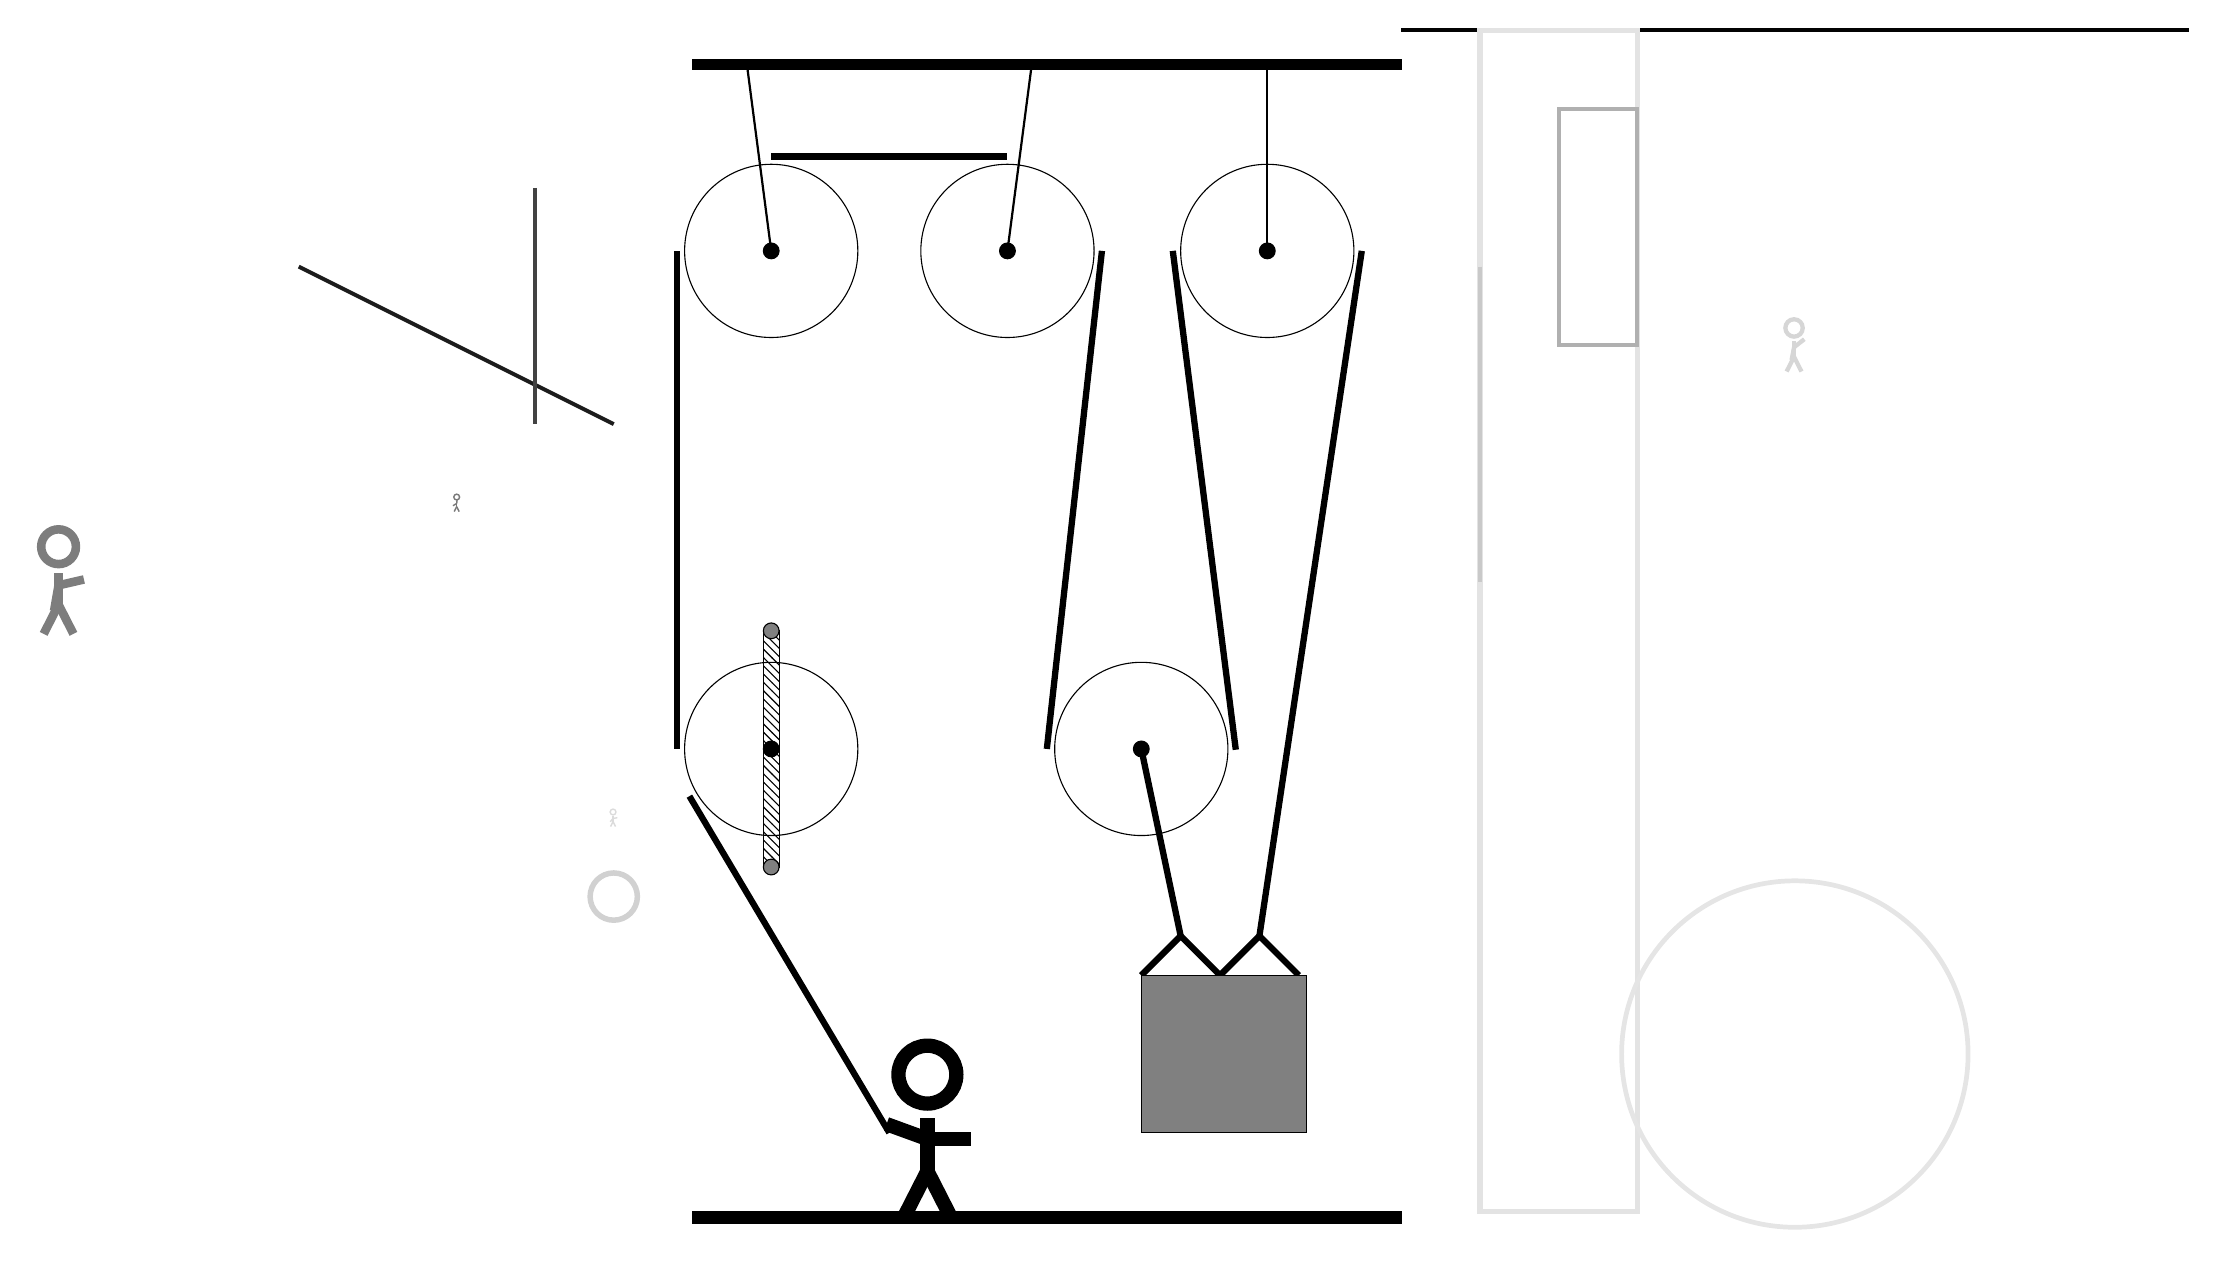
\begin{tikzpicture}
			%%%%% START %%%%%
			
			\draw[fill=black] (-3, 11.5) rectangle (6, 11.625);
			
			\draw (1, 9.2) circle (1.1);
			\draw[fill=black] (1, 9.2) circle (0.1);
			\draw[thick] (1, 9.2) -- (1.3, 11.5);
			
			\node[line width=0.2mm, color=black!16] at (11, 8) {\Strichmaxerl[3][79][38]};
			
			\draw [line width=0.7mm, color=black!18](-4, 1) circle (0.3);
			\draw[line width=0.5mm, color=black!99](6, 12) -- (16, 12);
			\node[line width=0.7mm, color=black!51] at (-11, 5) {\Strichmaxerl[6][80][13]};
			
			\draw[line width=0.7mm, color=black!11] (7, 12) rectangle (9, -3);
			\node[line width=0.7mm, color=black!14] at (-4, 2) {\Strichmaxerl[1][50][10]};
			\draw[line width=0.5mm, color=black!89](-8, 9) -- (-4, 7);
			\draw[line width=0.5mm, color=black!74](-5, 10) -- (-5, 7);
			\draw[line width=0.5mm, color=black!31] (8, 11) rectangle (9, 8);
			\draw [line width=0.6mm, color=black!10](11, -1) circle (2.2);
			\draw[line width=0.5mm, color=black!21](7, 9) -- (7, 5);
			
			\node[line width=0.6mm, color=black!52] at (-6, 6) {\Strichmaxerl[1][31][84]};
			
			\draw (4.3, 9.2) circle (1.1);
			\draw[fill=black] (4.3, 9.2) circle (0.1);
			\draw[thick] (4.3, 9.2) -- (4.3, 11.5);
			
			\draw (2.7, 2.875) circle (1.1);
			\draw[fill=black] (2.7, 2.875) circle (0.1);
			
			\draw[line width=0.8mm]  (2.7, 0.0) -- (3.2, 0.5) -- (3.7, 0.0) -- (4.2, 0.5) -- (4.7, 0.0);
			\draw[fill=black!50] (2.7, 0.0) rectangle (4.8, -2.0);
			
			\draw (-2, 9.2) circle (1.1);
			\draw[fill=black] (-2, 9.2) circle (0.1);
			\draw[thick] (-2, 9.2) -- (-2.3, 11.5);
			
			\draw (-2, 2.875) circle (1.1);
			\draw[fill=black] (-2, 2.875) circle (0.1);
			\draw[pattern=north west lines, pattern color=black] (-2.1, 4.375) rectangle (-1.9, 1.375);
			\draw[fill=black!50] (-2, 4.375) circle (0.1);
			\draw[fill=black!50] (-2, 1.375) circle (0.1);
			
			\draw[line width=0.8mm](-0.5, -2) -- (-3.0392, 2.275);
			\centerarc[line width=0.8mm](-2, 2.875)(180:210:1.2000000000000002);
			\draw[line width=0.8mm](-3.2, 2.875) -- (-3.2, 9.2);
			\centerarc[line width=0.8mm](-2, 9.2)(90:180:1.2000000000000002);
			
			\draw[line width=0.8mm](-2, 10.4) -- (1, 10.4);
			\centerarc[line width=0.8mm](1, 9.2)(0:90:1.2000000000000002);
			\draw[line width=0.8mm](2.2, 9.2) -- (1.5, 2.875);
			\centerarc[line width=0.8mm](2.7, 2.875)(180:370:1.2000000000000002);
			\draw[line width=0.8mm] (3.9, 2.865) -- (3.1, 9.2);
			\centerarc[line width=0.8mm](4.3, 9.2)(0:180:1.2000000000000002);
			\draw[line width=0.8mm](4.2, 0.5) -- (5.5, 9.2);
			\draw[line width=0.8mm] (3.2, 0.5) -- (2.7, 2.875);
			
			\node at (0, -2) {\Strichmaxerl[10][-20][0]};
			
			\draw[fill=black] (-3, -3) rectangle (6, -3.15);
			
			%%%%% END %%%%%
		\end{tikzpicture}
	\end{figure}	
\end{document}